\section* {1.1  LU -  разложение матриц}

\subsection{Постановка задачи}
Реализовать алгоритм LU -  разложения матриц (с выбором главного элемента) в виде программы. Используя разработанное программное обеспечение, решить систему линейных алгебраических уравнений (СЛАУ). Для матрицы СЛАУ вычислить определитель и обратную матрицу. 

{\bfseries Вариант:} 13

\begin{cases}
& -6x_1-5x_2-3x_3-8x_4 = 101 \\
& 5x_1-x_2-5x_3-4x_4 = 51 \\
& -6x_1+5x_3+5x_4 = -53 \\
& -7x_1-2x_2+8x_3+5x_4 = -63 \\
\end{cases}
%\pagebreak

\subsection{Результаты работы}
\begin{figure}[h!]
\centering
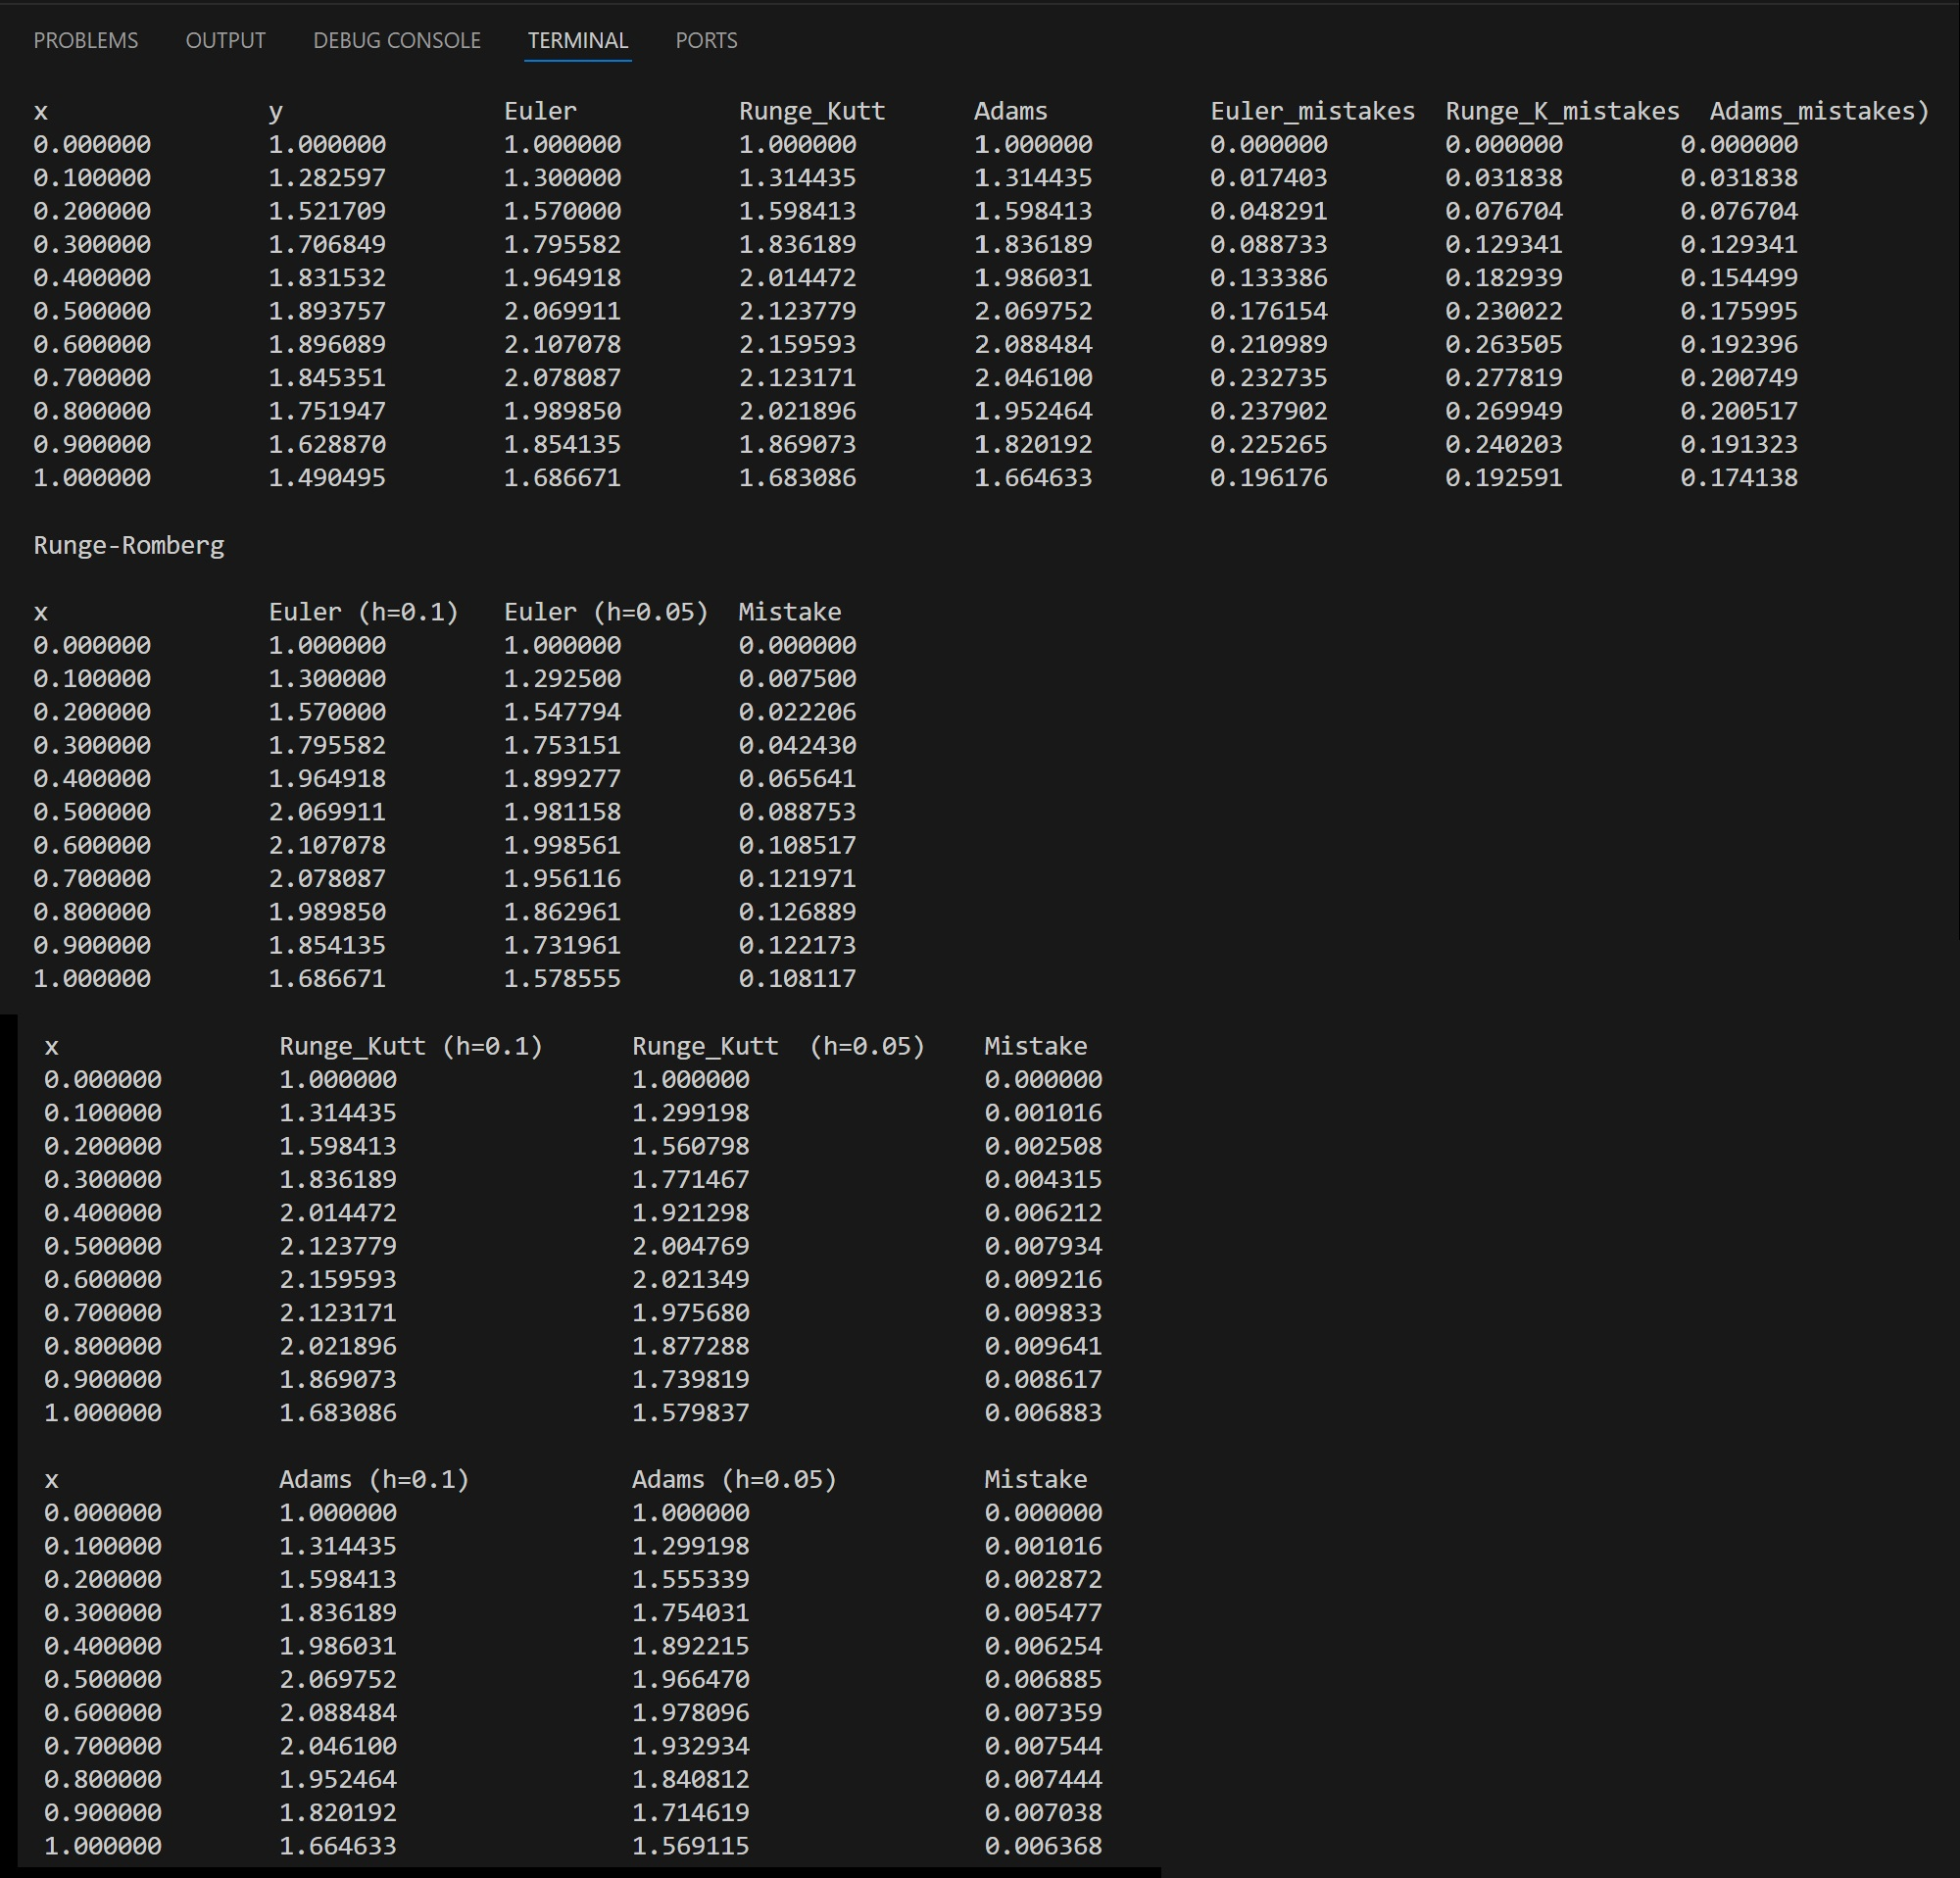
\includegraphics[width=15cm, height=10cm]{img_1}
\caption{Вывод программы в консоли}
\end{figure}
\pagebreak

\subsection{Исходный код}

\lstinputlisting{include/Lab_1.1.cpp}
\pagebreak
\section* {1.2  Метод прогонки}

\subsection{Постановка задачи}
Реализовать метод прогонки в виде программы, задавая в качестве входных данных ненулевые элементы матрицы системы и вектор правых частей. Используя разработанное программное обеспечение, решить СЛАУ с трехдиагональной матрицей.  

{\bfseries Вариант:} 13

\begin{cases}
& 14x_1-9x_2 = 125 \\
& -8x_1+14x_2+6x_3 = -56 \\
& -5x_2-17x_3+8x_4= 144 \\
& x_3+5x_4-2x_5 = 36 \\
& -4x_4-10x_5 = 70\\
\end{cases}
% \pagebreak

\subsection{Результаты работы}
\begin{figure}[h!]
\centering
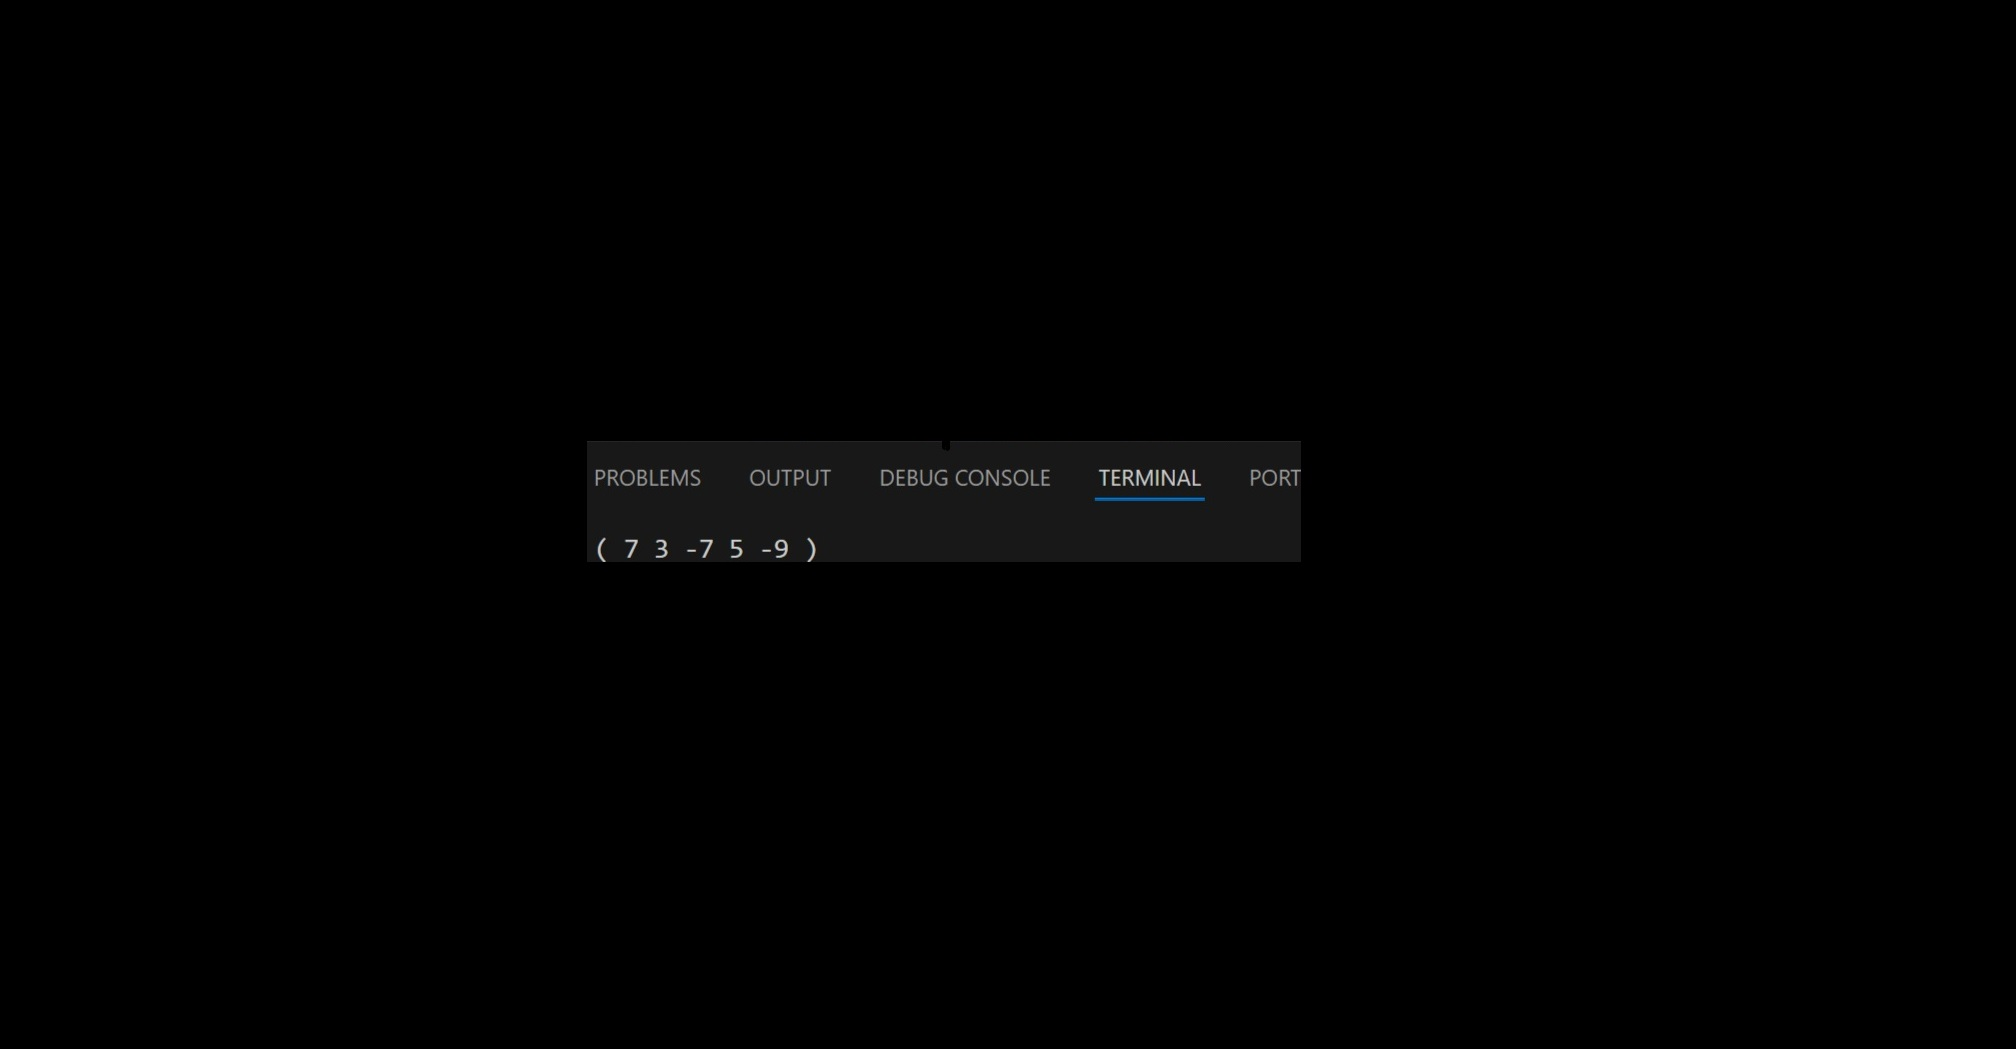
\includegraphics[width=.7\textwidth]{img_2}
\caption{Вывод программы в консоли}
\end{figure}
\pagebreak

\subsection{Исходный код}
\lstinputlisting{include/Lab_1.2.cpp}

\pagebreak
\section* {1.3  Метод простых итераций. Метод Зейделя}

\subsection{Постановка задачи}
Реализовать метод простых итераций и метод Зейделя в виде программ, задавая в качестве входных данных матрицу системы, вектор правых частей и точность вычислений. Используя разработанное программное обеспечение, решить СЛАУ. Проанализировать количество итераций, необходимое для достижения заданной точности. 

{\bfseries Вариант:} 13

\begin{cases}

& 24x_1-7x_2-4x_3+4x_4 = 190 \\
& -3x_1-9x_2-2x_3-2x_4 = -12 \\
& 3x_1+7x_2+24x_3+9x_4 = 155 \\
& x_1-6x_2-2x_3-15x_4 = -17 \\
\end{cases}
% \pagebreak

\subsection{Результаты работы}
\begin{figure}[h!]
\centering
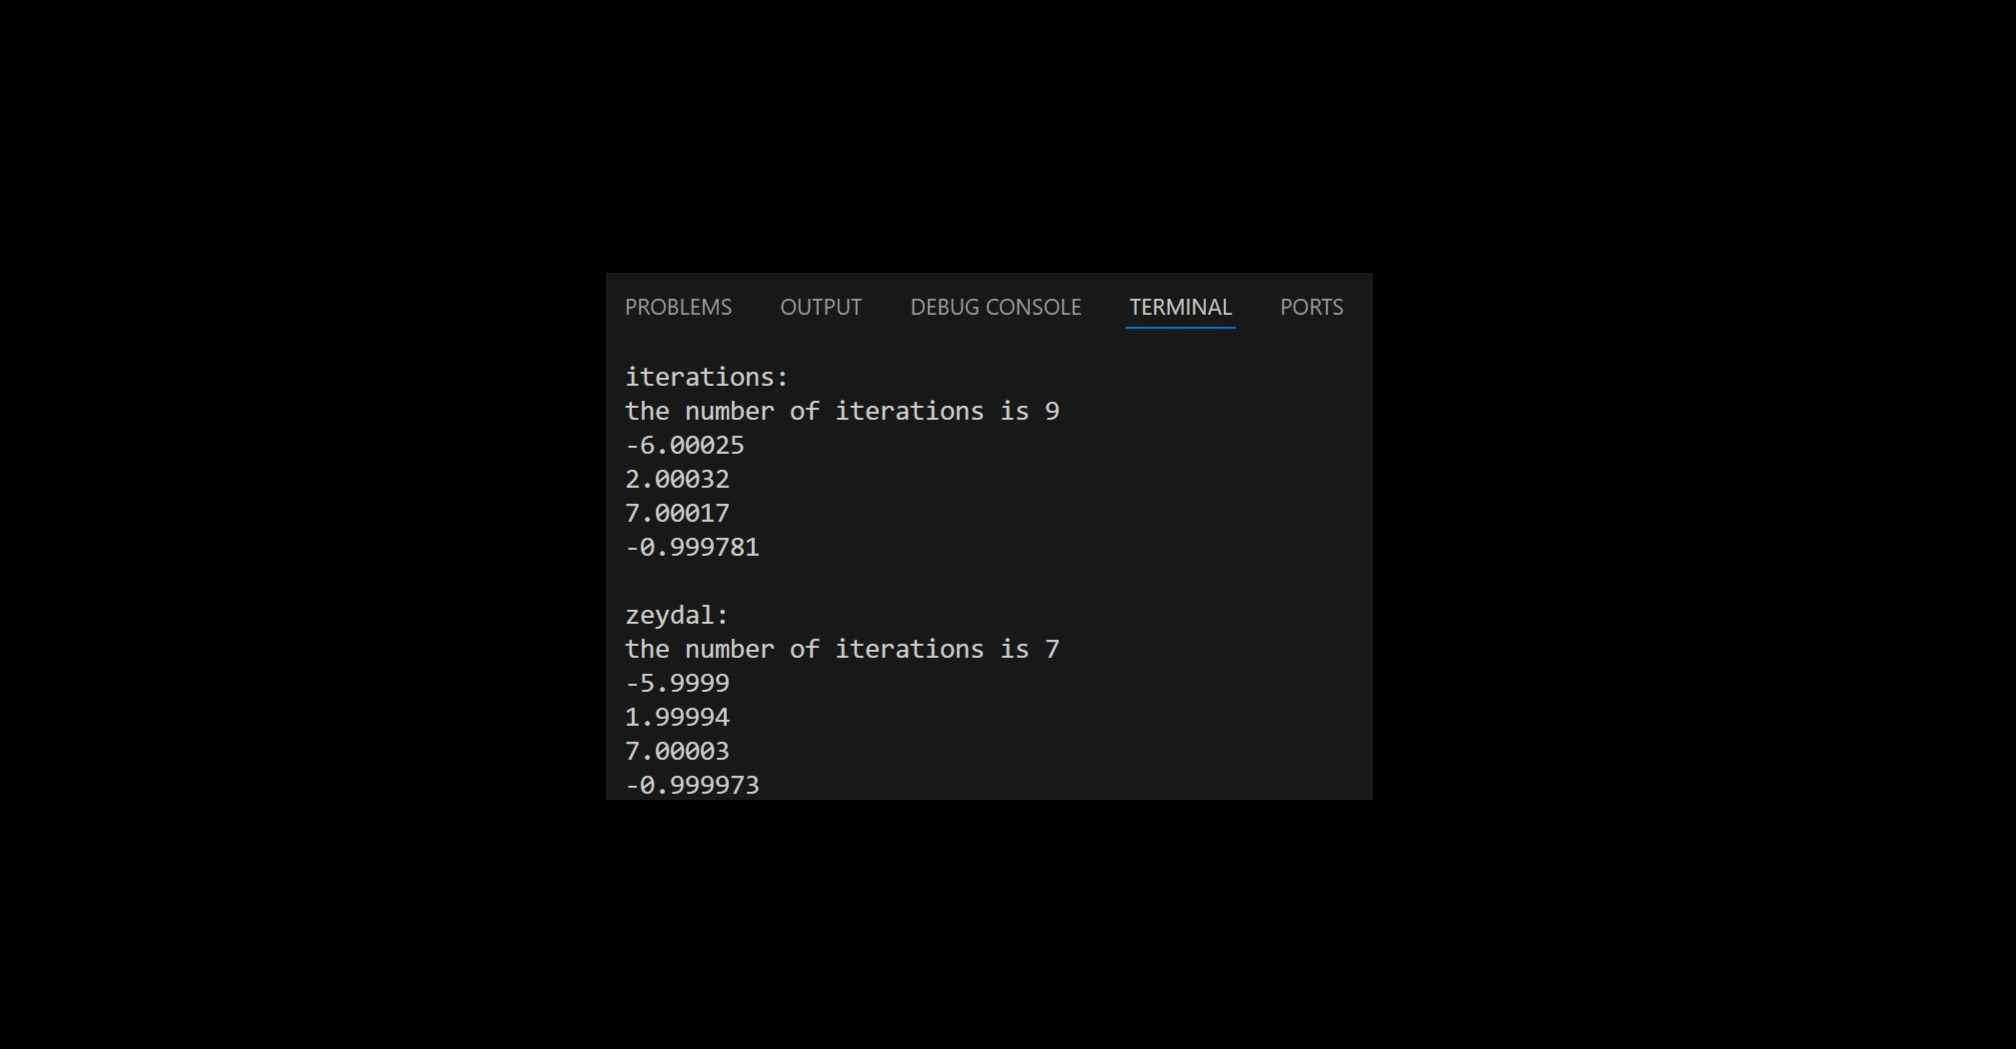
\includegraphics[width=15cm, height=10cm]{img_3}
\caption{Вывод программы в консоли}
\end{figure}

% \vfill

\pagebreak

\subsection{Исходный код}
\lstinputlisting{include/Lab_1.3.cpp}

\pagebreak
\section* {1.4  Метод вращений}

\subsection{Постановка задачи}
Реализовать метод вращений в виде программы, задавая в качестве входных данных матрицу и точность вычислений. Используя разработанное программное обеспечение, найти собственные значения и собственные векторы симметрических матриц. Проанализировать зависимость погрешности вычислений от числа итераций. 

{\bfseries Вариант:} 13

  \begin{pmatrix}
    8 & 0 & -2 \\
    0 & -5 & 4 \\
    -2 & 4 & -6
  \end{pmatrix}
% \pagebreak

\subsection{Результаты работы}
\begin{figure}[h!]
\centering
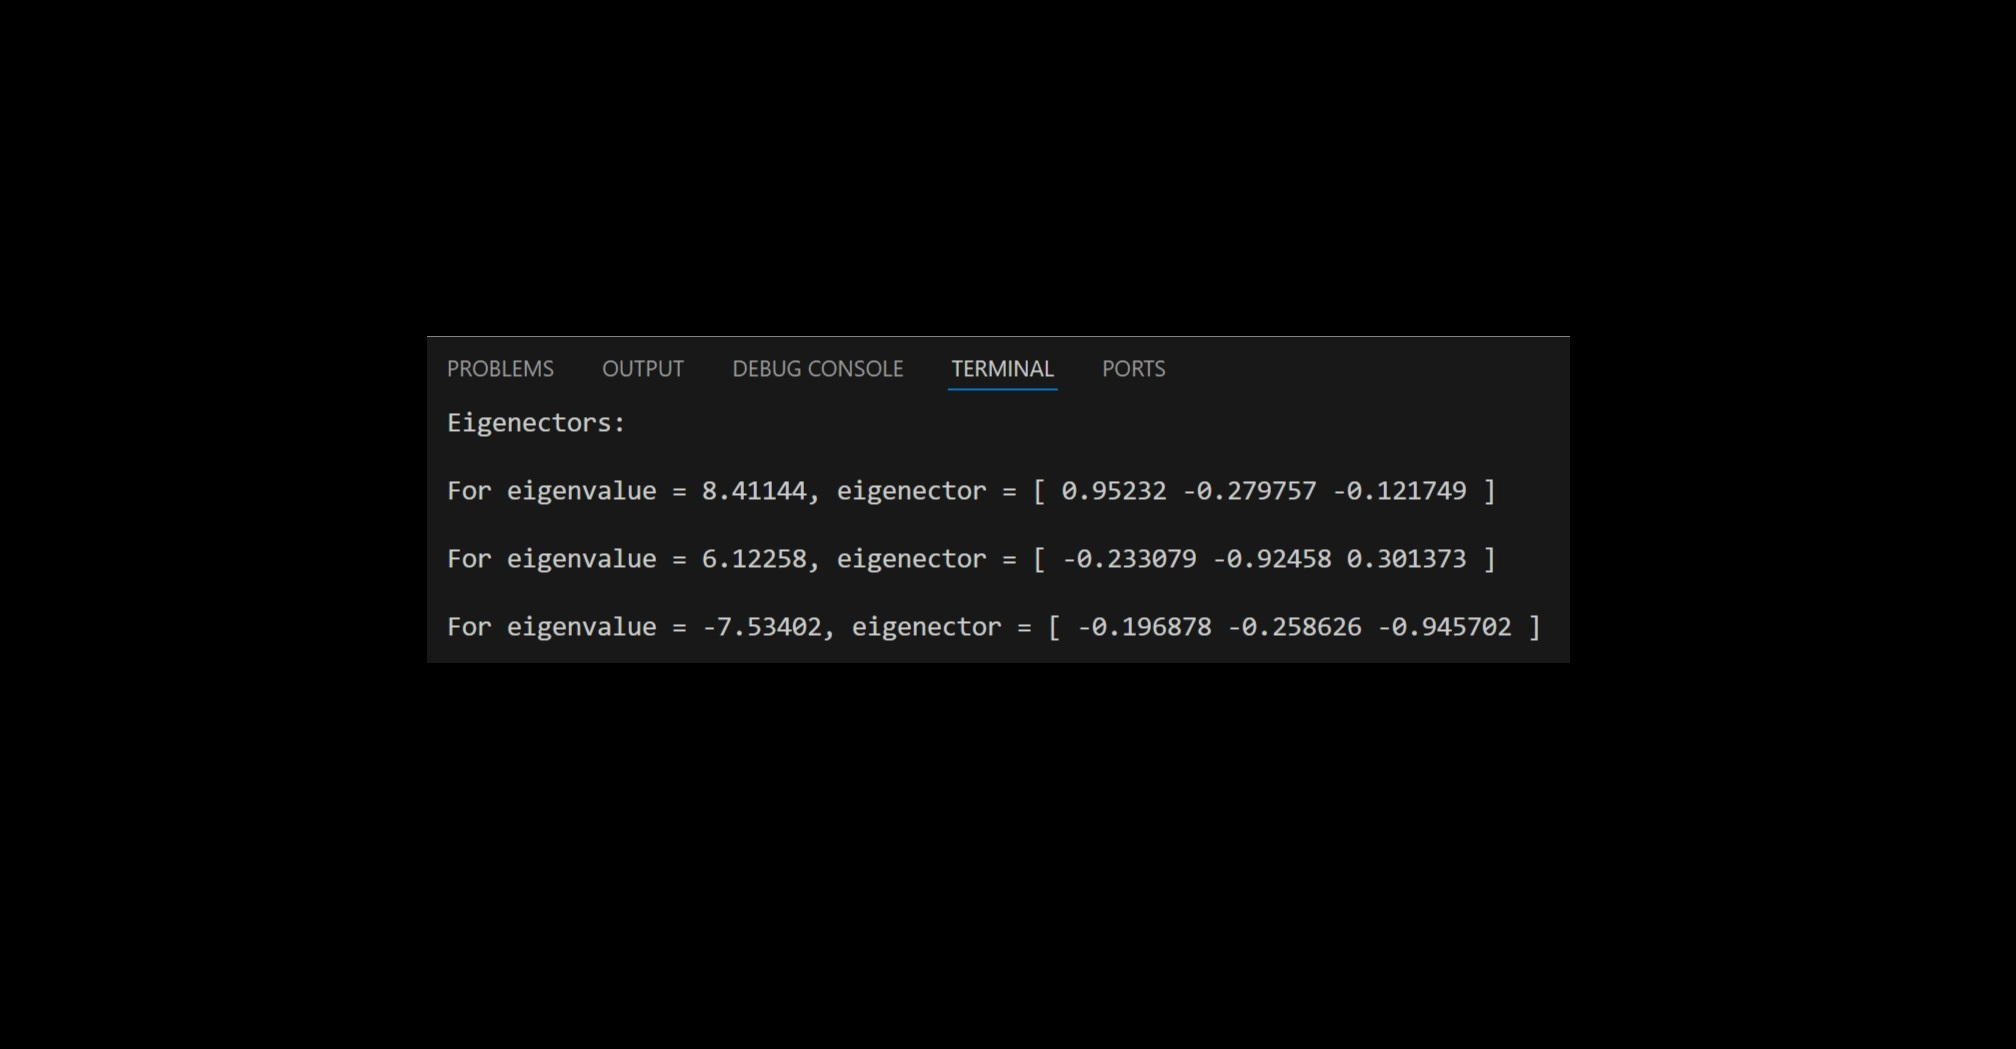
\includegraphics[width=.9\textwidth]{img_4}
\caption{Вывод программы в консоли}
\end{figure}

\pagebreak

\subsection{Исходный код}
\lstinputlisting{include/Lab_1.4.cpp}

\pagebreak
\section* {1.5  QR – разложение матриц}

\subsection{Постановка задачи}
Реализовать алгоритм QR – разложения матриц в виде программы. На его основе разработать программу, реализующую QR – алгоритм решения полной проблемы собственных значений произвольных матриц, задавая в качестве входных данных матрицу и точность вычислений. С использованием разработанного программного обеспечения найти собственные значения матрицы.


{\bfseries Вариант:} 13

  \begin{pmatrix}
    -1 & 2 & 9 \\
    9 & 3 & 4 \\
    8 & -4 & -6
  \end{pmatrix}
% \pagebreak

\subsection{Результаты работы}
\begin{figure}[h!]
\centering
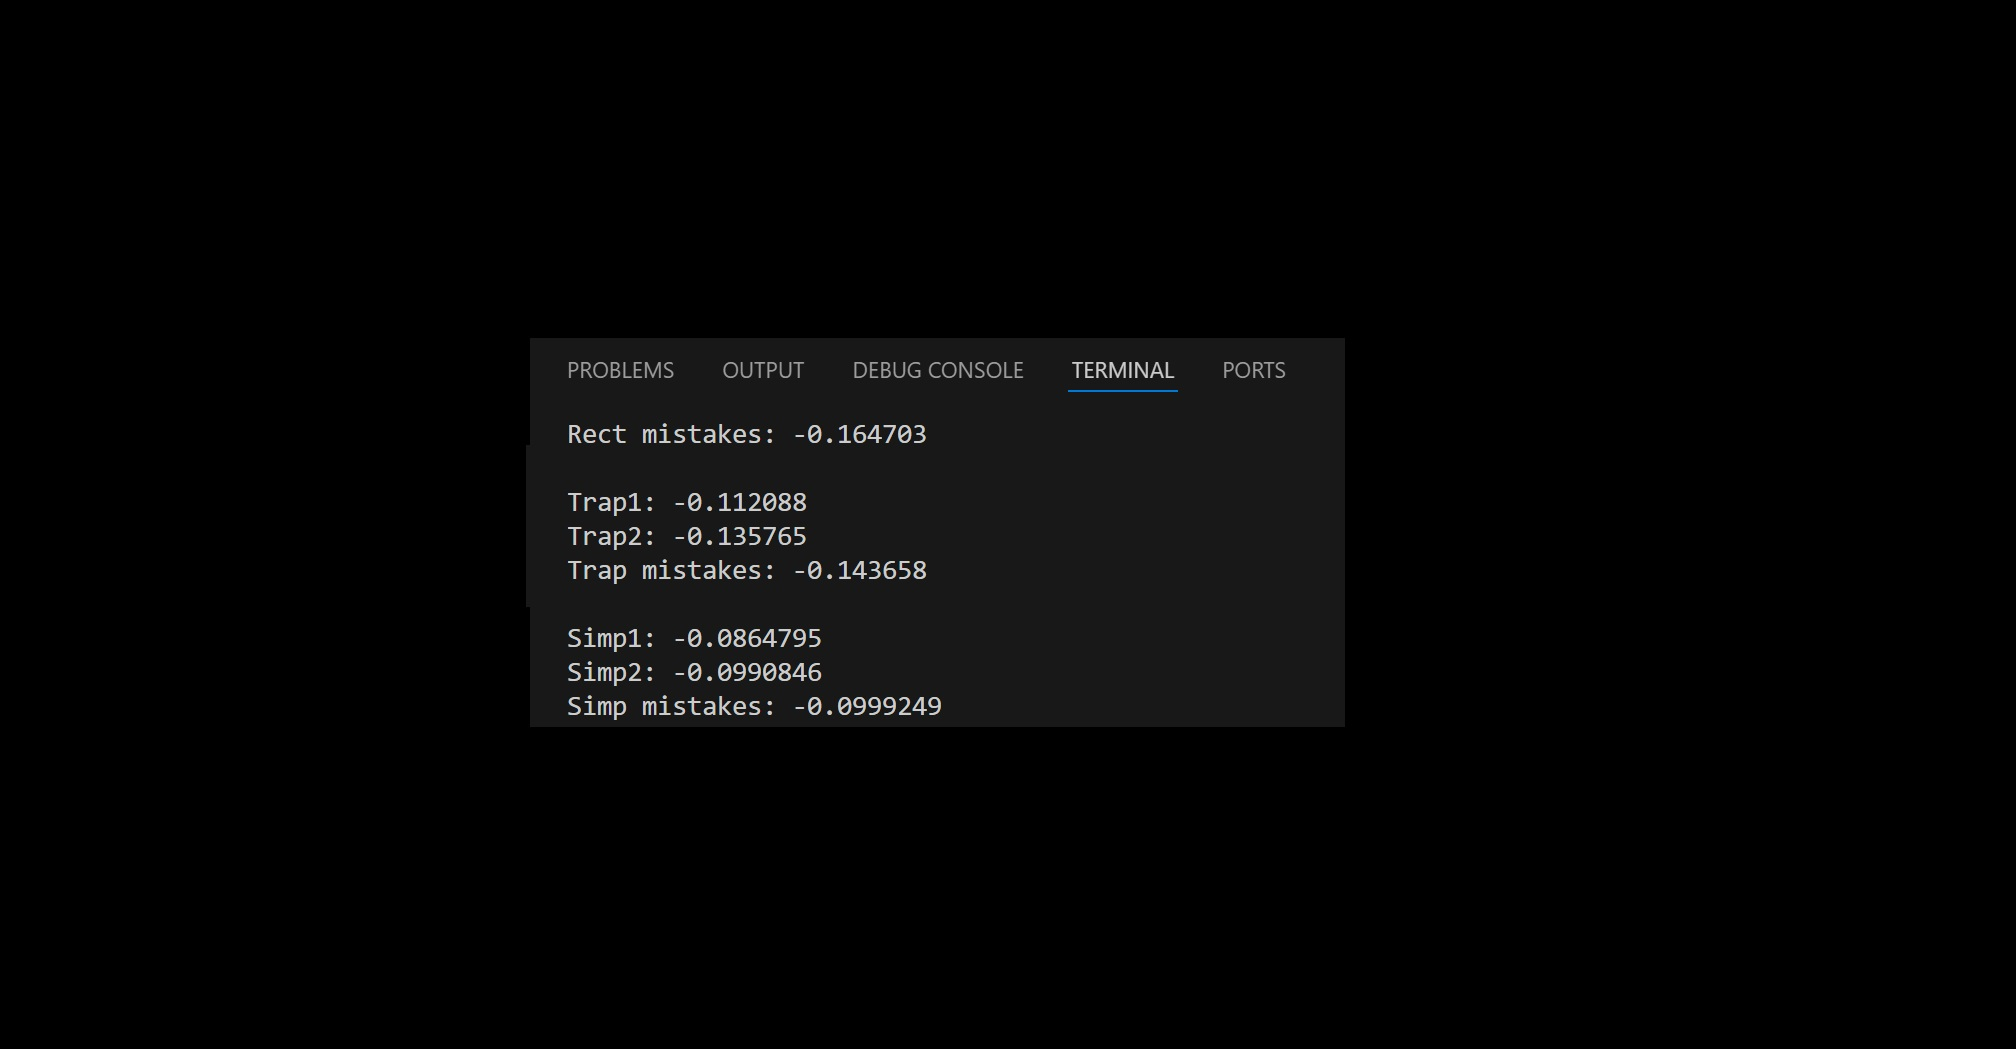
\includegraphics[width=.9\textwidth]{img_5}
\caption{Вывод программы в консоли}
\end{figure}

\pagebreak

\subsection{Исходный код}
\lstinputlisting{include/Lab_1.5.c}
